\documentclass[border=2mm]{standalone}
\usepackage{tikz}
\begin{document}

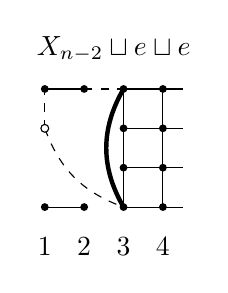
\begin{tikzpicture}[scale=0.5]
  % Draw structural lines (solid and dashed)
  \draw (1,1)--(2,1) (3,1)--(4.5,1) (1,4)--(2,4);
  \draw (3,2)--(4.5,2) (3,3)--(4.5,3) (3,4)--(4.5,4);
  \draw (3,1)--(3,4) (4,1)--(4,4);
  \draw [dashed] (2,4)--(3,4) (1,3)--(1,4);
  \draw [dashed] (1,3) to [out=290, in=160] (3,1);
  \draw [ultra thick] (3,1) to [out=120, in=240] (3,4);
  
  % Place filled circle nodes at data points
  \foreach \x in {1,2,3,4} {\node at (\x, 1) [fill,circle,inner sep=1pt] {};}
  \foreach \x in {3,4} {\node at (\x, 2) [fill,circle,inner sep=1pt] {};}
  \foreach \x in {1,3,4} {\node at (\x, 3) [fill,circle,inner sep=1pt] {};}
  \foreach \x in {1,2,3,4} {\node at (\x, 4) [fill,circle,inner sep=1pt] {};}
  
  % Overlay special node (white-filled circle) at (1,3) to highlight it
  \node at (1,3) [circle, draw=black, fill=white, inner sep=1pt] {};
  
  % Add axis labels and annotations
  \foreach \x in {1,2,3,4} {\node at (\x,0) {\x};}
  \node at (2.75,5) {$X_{n-2} \sqcup e \sqcup e$};
\end{tikzpicture}

\end{document}
